\documentclass[12pt]{article}

\usepackage{tabularx}
\usepackage{booktabs}
\usepackage{graphicx}
\usepackage{paralist}
\usepackage{listings}
\usepackage{booktabs}
\usepackage{hyperref}
\usepackage{amsfonts}
\usepackage{amsmath}
\usepackage{color}
\usepackage{fancyhdr}
\usepackage{geometry}
\usepackage{multirow}
\usepackage[round]{natbib}
\usepackage{fullpage}
\usepackage[round]{natbib}
\usepackage{float}

\newcounter{acnum}
\newcommand{\actheacnum}{AC\theacnum}
\newcommand{\acref}[1]{AC\ref{#1}}

\newcounter{ucnum}
\newcommand{\uctheucnum}{UC\theucnum}
\newcommand{\uref}[1]{UC\ref{#1}}

\newcounter{mnum}
\newcommand{\mthemnum}{M\themnum}
\newcommand{\mref}[1]{M\ref{#1}}

\geometry{margin = 0.75in}
\title{SE 3XA3: MG\\Space Invaders}

\begin{document}

\maketitle

%%%%%%%%%%%%%%%%%%%Team Information%%%%%%%%%%%%%%%%%%%%%%
{\Large Team Information:}
\begin{table}[htp]
\centering
{\Large
\begin{tabular}{|c|c|c|}
\hline
\multicolumn{1}{|l|}{Team Number} & Name         & MACID   \\ \hline
\multirow{3}{*}{L03 G07}          & Qianlin Chen & chenq84 \\ \cline{2-3} 
                                  & Jiacheng Wu  & wuj187  \\ \cline{2-3} 
                                  & Tingyu Shi   & shit19  \\ \hline
\end{tabular}
}
\end{table}

%%%%%%%%%%% Revision History%%%%%%%%%%%%%
\newpage
\begin{table}[htp]
\caption{Revision History} 
\begin{tabularx}{\textwidth}{llX}
\toprule
\textbf{Date} & \textbf{Developer(s)} & \textbf{Change}\\
\midrule
January 26, 2022 & All team members & Initial Document\\
March 18, 2022 & Qianlin Chen & Section3, section5\\
March 10, 2022 & Jiacheng Wu & Section1, Section2, Section5, Section6\\
March 10, 2022 & Tingyu Shi & Section4, Section7\\
\bottomrule
\end{tabularx}
\end{table}
\newpage
%%%%%%%%%%%%%%Contents%%%%%%%%%%%%%%%%
\tableofcontents
\listoftables
\listoffigures
\cleardoublepage

\section{Introduction}
Space Invader is a video game that player will control an aircraft to eliminate all the monsters. The goal of the project is to upgrade the graphics of the game. Additionally, we will use software engineering principle to redevelop it.

\subsection{Purpose}
The purpose of this document is to demonstrate the modular representation of the system in order to separate the concerns and hide the information. The document also provide high cohesion and low coupling to reduce the complexity of the system.

\subsection{Scope}
The Module guide will provides all the modules that based on the requirements in the SRS document. Also, the external behaviours of the modules will go into the MIS documents.
\newpage
\subsection{Acronyms, Abbreviations, and Symbols}
	
\begin{table}[hbp]
\caption{\textbf{Table of Abbreviations}}

\begin{tabularx}{\textwidth}{p{3cm}X}
\toprule
\textbf{Abbreviation} & \textbf{Definition} \\
\midrule
SRS & Software requirement specification\\\\
PC & personal computer\\\\
FPS & frams per second\\\\
GUI & graphic user interface\\\\
HP & health point of the aircraft\\\\

\bottomrule
\end{tabularx}



\caption{\textbf{Table of Definitions}}

\begin{tabularx}{\textwidth}{p{3cm}X}
\toprule
\textbf{Term} & \textbf{Definition}\\
\midrule
Space invader & The name of a video game\\\\
Graphic User Interface & a graphic representation for users to interact\\\\
Score & The number that represents the achivement of users\\\\
Players & the users of the game that follow certain rules to succeed\\\\
Aircraft & the users will controll the aircraft to play the game\\\\
Monster & the goal of the game, the target the aircraft to attack.\\\\
items & the element in game that can boost users' ammo\\\\
\bottomrule
\end{tabularx}

\end{table}	




\subsection{Overview of Document}
The rest of the document is organized as follows. Section
\ref{SecChange} lists the anticipated and unlikely changes of the software
requirements. Section \ref{SecMH} summarizes the module decomposition that
was constructed according to the likely changes. Section \ref{SecConnection}
specifies the connections between the software requirements and the
modules. Section \ref{SecMD} gives a detailed description of the
modules. Section \ref{SecTM} includes two traceability matrices. One checks
the completeness of the design against the requirements provided in the SRS. The
other shows the relation between anticipated changes and the modules. Section
\ref{SecUse} describes the use relation between modules.

\section{Anticipated and Unlikely Changes} \label{SecChange}

This section lists possible changes to the system. According to the likeliness
of the change, the possible changes are classified into two
categories. Anticipated changes are listed in Section \ref{SecAchange}, and
unlikely changes are listed in Section \ref{SecUchange}.

\subsection{Anticipated Changes} \label{SecAchange}

Anticipated changes are the source of the information that is to be hidden
inside the modules. Ideally, changing one of the anticipated changes will only
require changing the one module that hides the associated decision. The approach
adapted here is called design for
change.

\begin{description}
\item[\refstepcounter{acnum} \actheacnum :] The data structure to represent the monster.
\item[\refstepcounter{acnum} \actheacnum :] The algorithm to determine the collision between bullets, monsters, obstacles and the aircraft.
\item [\refstepcounter{acnum} \actheacnum :]The visual effect when collisions happen.
\item [\refstepcounter{acnum} \actheacnum :]How the scores are calculated.
\item [\refstepcounter{acnum} \actheacnum :]Soundtrack of the game.
\item [\refstepcounter{acnum} \actheacnum :]The algorithm to represent shooting bullets.
\end{description}

\subsection{Unlikely Changes} \label{SecUchange}

The module design should be as general as possible. However, a general system is
more complex. Sometimes this complexity is not necessary. Fixing some design
decisions at the system architecture stage can simplify the software design. If
these decision should later need to be changed, then many parts of the design
will potentially need to be modified. Hence, it is not intended that these
decisions will be changed.

\begin{description}
\item[\refstepcounter{ucnum} \uctheucnum :] Input/Output devices: The game only focuses on keyboard as input and screen as output.
\item[\refstepcounter{ucnum} \uctheucnum :] There will always be
  a source of input data external to the software.
\item[\refstepcounter{ucnum} \uctheucnum :] The software architecture of the game since the PAC is the best option for this design.
\item[\refstepcounter{ucnum} \uctheucnum :] The running environment of the game.(WIN,MACOS,LINUX)
\end{description}

\section{Module Hierarchy} \label{SecMH}
This section provides an overview of the module design. Modules are summarized in a hierarchy decomposed by secrets in Table \ref{TblMH}. The modules listed below, which are leaves in the hierarchy tree, are the modules that will actually be implemented.

\begin{description}
\item [\refstepcounter{mnum} \mthemnum \label{m1}:] SingleController
\item [\refstepcounter{mnum} \mthemnum \label{m2}:] DoubleController
\item [\refstepcounter{mnum} \mthemnum \label{m3}:] TotalController
\item [\refstepcounter{mnum} \mthemnum \label{m4}:] MonsterDisplay
\item [\refstepcounter{mnum} \mthemnum \label{m5}:] SpaceShipDisplay
\item [\refstepcounter{mnum} \mthemnum \label{m6}:] MonsterMatrixDisplay
\item [\refstepcounter{mnum} \mthemnum \label{m7}:] BulletDisplay
\item [\refstepcounter{mnum} \mthemnum \label{m8}:] ScoreDisplay
\item [\refstepcounter{mnum} \mthemnum \label{m9}:] ObstaclesDisplay
\item [\refstepcounter{mnum} \mthemnum \label{m10}:] AmmoDisplay
\item [\refstepcounter{mnum} \mthemnum \label{m11}:] HeartDisplay
\item [\refstepcounter{mnum} \mthemnum \label{m12}:] BombDisplay
\item [\refstepcounter{mnum} \mthemnum \label{m13}:] SetUpDisplay
\item [\refstepcounter{mnum} \mthemnum \label{m14}:] Monster 
\item [\refstepcounter{mnum} \mthemnum \label{m15}:] SpaceShip
\item [\refstepcounter{mnum} \mthemnum \label{m16}:] MonsterMatrix 
\item [\refstepcounter{mnum} \mthemnum \label{m17}:] Bullet
\item [\refstepcounter{mnum} \mthemnum \label{m18}:] Score
\item [\refstepcounter{mnum} \mthemnum \label{m19}:] Obstacle
\item [\refstepcounter{mnum} \mthemnum \label{m20}:] BulletState
\item [\refstepcounter{mnum} \mthemnum \label{m21}:] MonsterColor
\item [\refstepcounter{mnum} \mthemnum \label{m22}:] Ammo 
\item [\refstepcounter{mnum} \mthemnum \label{m23}:] Heart 
\item [\refstepcounter{mnum} \mthemnum \label{m24}:] Bomb 
\item [\refstepcounter{mnum} \mthemnum \label{m25}:] CollisionDetection
\item [\refstepcounter{mnum} \mthemnum \label{m25}:] Driver
\end{description}


\begin{table}[H]
\centering
\begin{tabular}{p{0.3\textwidth} p{0.6\textwidth}}
\toprule
\textbf{Level 1} & \textbf{Level 2}\\
\midrule

{Hardware-Hiding Module} & ~ \\
& ~ \\
\midrule

{Behaviour-Hiding Module} & SingleController\\
& DoubleController\\
& TotalController \\
& MonsterDisplay \\
& SpaceShipDisplay \\
& MonsterMatrixDisplay \\ 
& BulletDisplay \\
& ScoreDisplay \\
& ObstaclesDisplay\\
& AmmoDisplay\\
& HeartDisplay\\
& BombDisplay\\
& SetUpDisplay\\
& Driver\\
\midrule

{Software Decision Module} & Monster\\
& SpaceShip\\
& MonsterMatrix\\
& Bullet\\
& Score\\
& Obstacle\\
& BulletState\\
& MonsterColor\\
& Ammo\\
& Heart\\
& Bomb\\
& CollisionDetection\\
\bottomrule

\end{tabular}
\caption{Module Hierarchy}
\label{TblMH}
\end{table}
\section{Connection Between Requirements and Design} \label{SecConnection}

The design of the system is intended to satisfy the requirements developed in
the SRS. In this stage, the system is decomposed into modules. The connection
between requirements and modules is listed in Table \ref{TblRT}.

\section{Module Decomposition} \label{SecMD}

Modules are decomposed according to the principle of ``information hiding''
proposed by Parnas The \emph{Secrets} field in a module
decomposition is a brief statement of the design decision hidden by the
module. The \emph{Services} field specifies \emph{what} the module will do
without documenting \emph{how} to do it. For each module, a suggestion for the
implementing software is given under the \emph{Implemented By} title. If the
entry is \emph{OS}, this means that the module is provided by the operating
system or by standard programming language libraries.  Also indicate if the
module will be implemented specifically for the software.
\\
\noindent 
Only the leaf modules in the
hierarchy have to be implemented. If a dash (\emph{--}) is shown, this means
that the module is not a leaf and will not have to be implemented. Whether or
not this module is implemented depends on the programming language
selected.

\subsection{Hardware Hiding Modules}

N/A

\subsection{Behaviour-Hiding Module}

\subsubsection{Driver(M26)}
\textbf{Secrets:} Actions to do to inilialize the total controller.\\\\
\textbf{Service:} Initialize the total controller.\\\\
\textbf{Implemented By:} Space Invader

\subsubsection{SingleController(M1)}

\textbf{Secrets:} Actions to be done after the user select single mode.\\\\
\textbf{Service:} Once single mode is selected, the user will play with one aircraft in the game.\\\\
\textbf{Implemented By:} Space Invader

\subsubsection{DoubleController(M2)}

\begin{description}
\item[Secrets:]Actions to be done after the user select double mode.
\item[Services:]Once double mode is selected, the users will play with two aircraft in the game.
\item[Implemented By:] Space Invader
\end{description}

\subsubsection{TotalController(M3)}
\begin{description}
\item[Secrets:] Actions the system do to provide single mode and double mode for users.
\item[Services:] Allow the users to select between single mode and double mode.
\item[Implemented By:] Space Invader
\end{description}

\subsubsection{MonsterDisplay(M4)}
\begin{description}
\item[Secrets:] The method to visualize a single monster.
\item[Services:] Display a monster on the screen and update the visualization as its model changes
\item[Implemented By:] Space Invader
\end{description}

\subsubsection{SpaceShipDisplay(M5)}
\begin{description}
\item[Secrets:] The method to visualize the aircraft.
\item[Services:] Display the aircraft on the screen and allow users to controll and display the change after user giving inputs.
\item[Implemented By:] Space Invader
\end{description}

\subsubsection{MonsterMatrixDisplay(M6)}
\begin{description}
\item[Secrets:] The method to visualize over one monsters.
\item[Services:] Display a number of monsters on the screen and update their visualization as their model change.
\item[Implemented By:] Space Invader
\end{description}

\subsubsection{BulletDisplay(M7)}
\begin{description}
\item[Secrets:] The method to visualize bullets.
\item[Services:] Display bullets on the screen and update their visualization as their model change.
\item[Implemented By:] Space Invader
\end{description}

\subsubsection{ScoreDisplay(M8)}
\begin{description}
\item[Secrets:] The method to visualize scores.
\item[Services:] Display scores on the screen and update their visualization as their model change.
\item[Implemented By:] Space Invader
\end{description}

\subsubsection{ObstaclesDisplay(M9)}
\begin{description}
\item[Secrets:] The method to visualize Obstacles.
\item[Services:] Display Obstacles on the screen and update their visualization as its model change.
\item[Implemented By:] Space Invader
\end{description}

\subsubsection{AmmoDisplay(M10)}
\begin{description}
\item[Secrets:] The method to visualize ammo items.
\item[Services:] Display ammo items on the screen and update their visualization as its model change.
\item[Implemented By:] Space Invader
\end{description}

\subsubsection{HeartDisplay(M11)}
\begin{description}
\item[Secrets:] The method to visualize Heart items.
\item[Services:] Display Heart items on the screen and update their visualization as its model change.
\item[Implemented By:] Space Invader
\end{description}

\subsubsection{BombDisplay(M12)}
\begin{description}
\item[Secrets:] The method to visualize Bomb items.
\item[Services:] Display Bomb items on the screen and update their visualization as its model change.
\item[Implemented By:] Space Invader
\end{description}

\subsubsection{SetUpDisplay(M13)}
\begin{description}
\item[Secrets:] The method to display welcoming message, game mode selection message, game instructions and game addiction prevention message.
\item[Services:]Display welcoming message, game mode selection message, game instructions and game addiction prevention message.
\item[Implemented By:] Space Invader
\end{description}

\subsection{Software Decision Module}

\subsubsection{Monster(M14)}
\begin{description}
\item[Secrets:] Data structures used to represent a monster and algorithms to change its states.
\item[Services:] Provide methods to represent a monster. 
\item[Implemented By:] Space Invader
\end{description}

\subsubsection{SpaceShip(M15)}
\begin{description}
\item[Secrets:] Data structures used to represent the aircraft and algorithms to change its states.
\item[Services:] Provide methods to represent the aircraft. 
\item[Implemented By:] Space Invader
\end{description}

\subsubsection{MonsterMatrix(M16)}
\begin{description}
\item[Secrets:] Data structures used to represent a number of monsters.
\item[Services:] Provide methods to represent over one monsters. 
\item[Implemented By:] Space Invader
\end{description}

\subsubsection{Bullet(M17)}
\begin{description}
\item[Secrets:] Data structures used to represent bullets and algorithms to change their states.
\item[Services:] Provide methods to represent bullets. 
\item[Implemented By:] Space Invader
\end{description}

\subsubsection{Score(M18)}
\begin{description}
\item[Secrets:] Algorithm to calculate the scores.
\item[Services:] Provide methods to determine the calculation of scores. 
\item[Implemented By:] Space Invader
\end{description}

\subsubsection{Obstacle(M19)}
\begin{description}
\item[Secrets:] Data structures used to represent Obstacles and algorithms to change their states.
\item[Services:] Provide methods to represent Obstacles. 
\item[Implemented By:] Space Invader
\end{description}

\subsubsection{BulletState(M20)}
\begin{description}
\item[Secrets:] Data used to represent bullet state.
\item[Services:] Provide different states for bullets. 
\item[Implemented By:] Space Invader
\end{description}

\subsubsection{MonsterColor(M21)}
\begin{description}
\item[Secrets:] Data used to represent monster color.
\item[Services:] Provide different colors for monsters. 
\item[Implemented By:] Space Invader
\end{description}

\subsubsection{Ammo(M22)}
\begin{description}
\item[Secrets:] Data structure used to represent ammo item and algorithms to represent its usage.
\item[Services:] Provide methods to represent ammo items and actions to change the ammo of the aircraft. 
\item[Implemented By:] Space Invader
\end{description}

\subsubsection{Heart(M23)}
\begin{description}
\item[Secrets:] Data structure used to represent heart item and algorithms to represent its usage.
\item[Services:] Provide methods to represent heart items and actions to change hp of the aircraft. 
\item[Implemented By:] Space Invader
\end{description}

\subsubsection{Bomb(M24)}
\begin{description}
\item[Secrets:] Data structure used to represent bomb item and algorithms to represent its usage.
\item[Services:] Provide methods to represent bomb items and actions to change states of monsters/obstacles. 
\item[Implemented By:] Space Invader
\end{description}

\subsubsection{CollisionDetection(M25)}
\begin{description}
\item[Secrets:] Algorithms to dectect if two objects in game overlap
\item[Services:] provide methods to determine if two objects collide
\item[Implemented By:] Space Invader
\end{description}
\newpage
\section{Traceability Matrix} \label{SecTM}
This section shows two traceability matrices: between the modules and the
requirements and between the modules and the anticipated changes.

% \begin{comment}
% the table should use mref, the requirements should be named, use something
% like fref
\begin{table}[H]
\centering
\begin{tabular}{p{0.2\textwidth} p{0.6\textwidth}}
\toprule
\textbf{Req.} & \textbf{Modules}\\
\midrule
FR1-FR3 & \mref{m13}\\
FR4 & \mref{m8}, \mref{m18}, \mref{m13}\\
FR5 & \mref{m15}, \mref{m13}\\
FR6 & \mref{m13}\\
FR7 & \mref{m6}, \mref{m13}\\
FR8 & \mref{m10}, \mref{m11}, \mref{m12}, \mref{m13}\\
FR9 & \mref{m5}, \mref{m13}\\
FR10 & \mref{m19}, \mref{m13}\\
FR11 & \mref{m18}, \mref{m13}\\
FR12-FR14 & \mref{m13}\\
FR15 & \mref{m8}\\
FR16 & \mref{m23}, \mref{m15}\\
FR17 & \mref{m3}\\
FR18-FR22 & \mref{m16}\\
FR23-FR27 & \mref{m14}\\
FR28 & \mref{m4}\\
FR29 & \mref{m19}\\
FR30-FR31 & \mref{m22}, \mref{m23}, \mref{m24}\\
FR32 & \mref{m16}, \mref{m14}, \mref{m24}\\
FR33 & \mref{m22}, \mref{m5}, \mref{m7}\\
FR34 & \mref{m23}, \mref{m5}\\
FR35 & \mref{m22}, \mref{m23}, \mref{m24},, \mref{m16}\\
FR36-FR39 & \mref{m3}\\
FR 40 & \mref{m15}\\

\bottomrule
\end{tabular}
\caption{Trace Between Requirements and Modules}
\label{TblRT}
\end{table}

\begin{table}[H]
\centering
\begin{tabular}{p{0.2\textwidth} p{0.6\textwidth}}
\toprule
\textbf{AC} & \textbf{Modules}\\
\midrule
AC1 & \mref{m14}\\
AC2 & \mref{m25}\\
AC3 & \mref{m4}, \mref{m6}\\
AC4 & \mref{m18}\\
AC5 & \mref{m3}\\
AC6 & \mref{m17}\\
\bottomrule
\end{tabular}
\caption{Trace Between Anticipated Changes and Modules}
\label{TblACT}
\end{table}
\newpage
\section{Use Hierarchy Between Modules} \label{SecUse}
In this section, the uses hierarchy between modules is
provided. Parnas(1978) said of two programs A and B that A {\em uses} B if
correct execution of B may be necessary for A to complete the task described in
its specification. That is, A {\em uses} B if there exist situations in which
the correct functioning of A depends upon the availability of a correct
implementation of B.  Figure \ref{FigUH} illustrates the use relation between
the modules. It can be seen that the graph is a directed acyclic graph
(DAG). Each level of the hierarchy offers a testable and usable subset of the
system, and modules in the higher level of the hierarchy are essentially simpler
because they use modules from the lower levels.

\begin{figure}[h!]
\centering
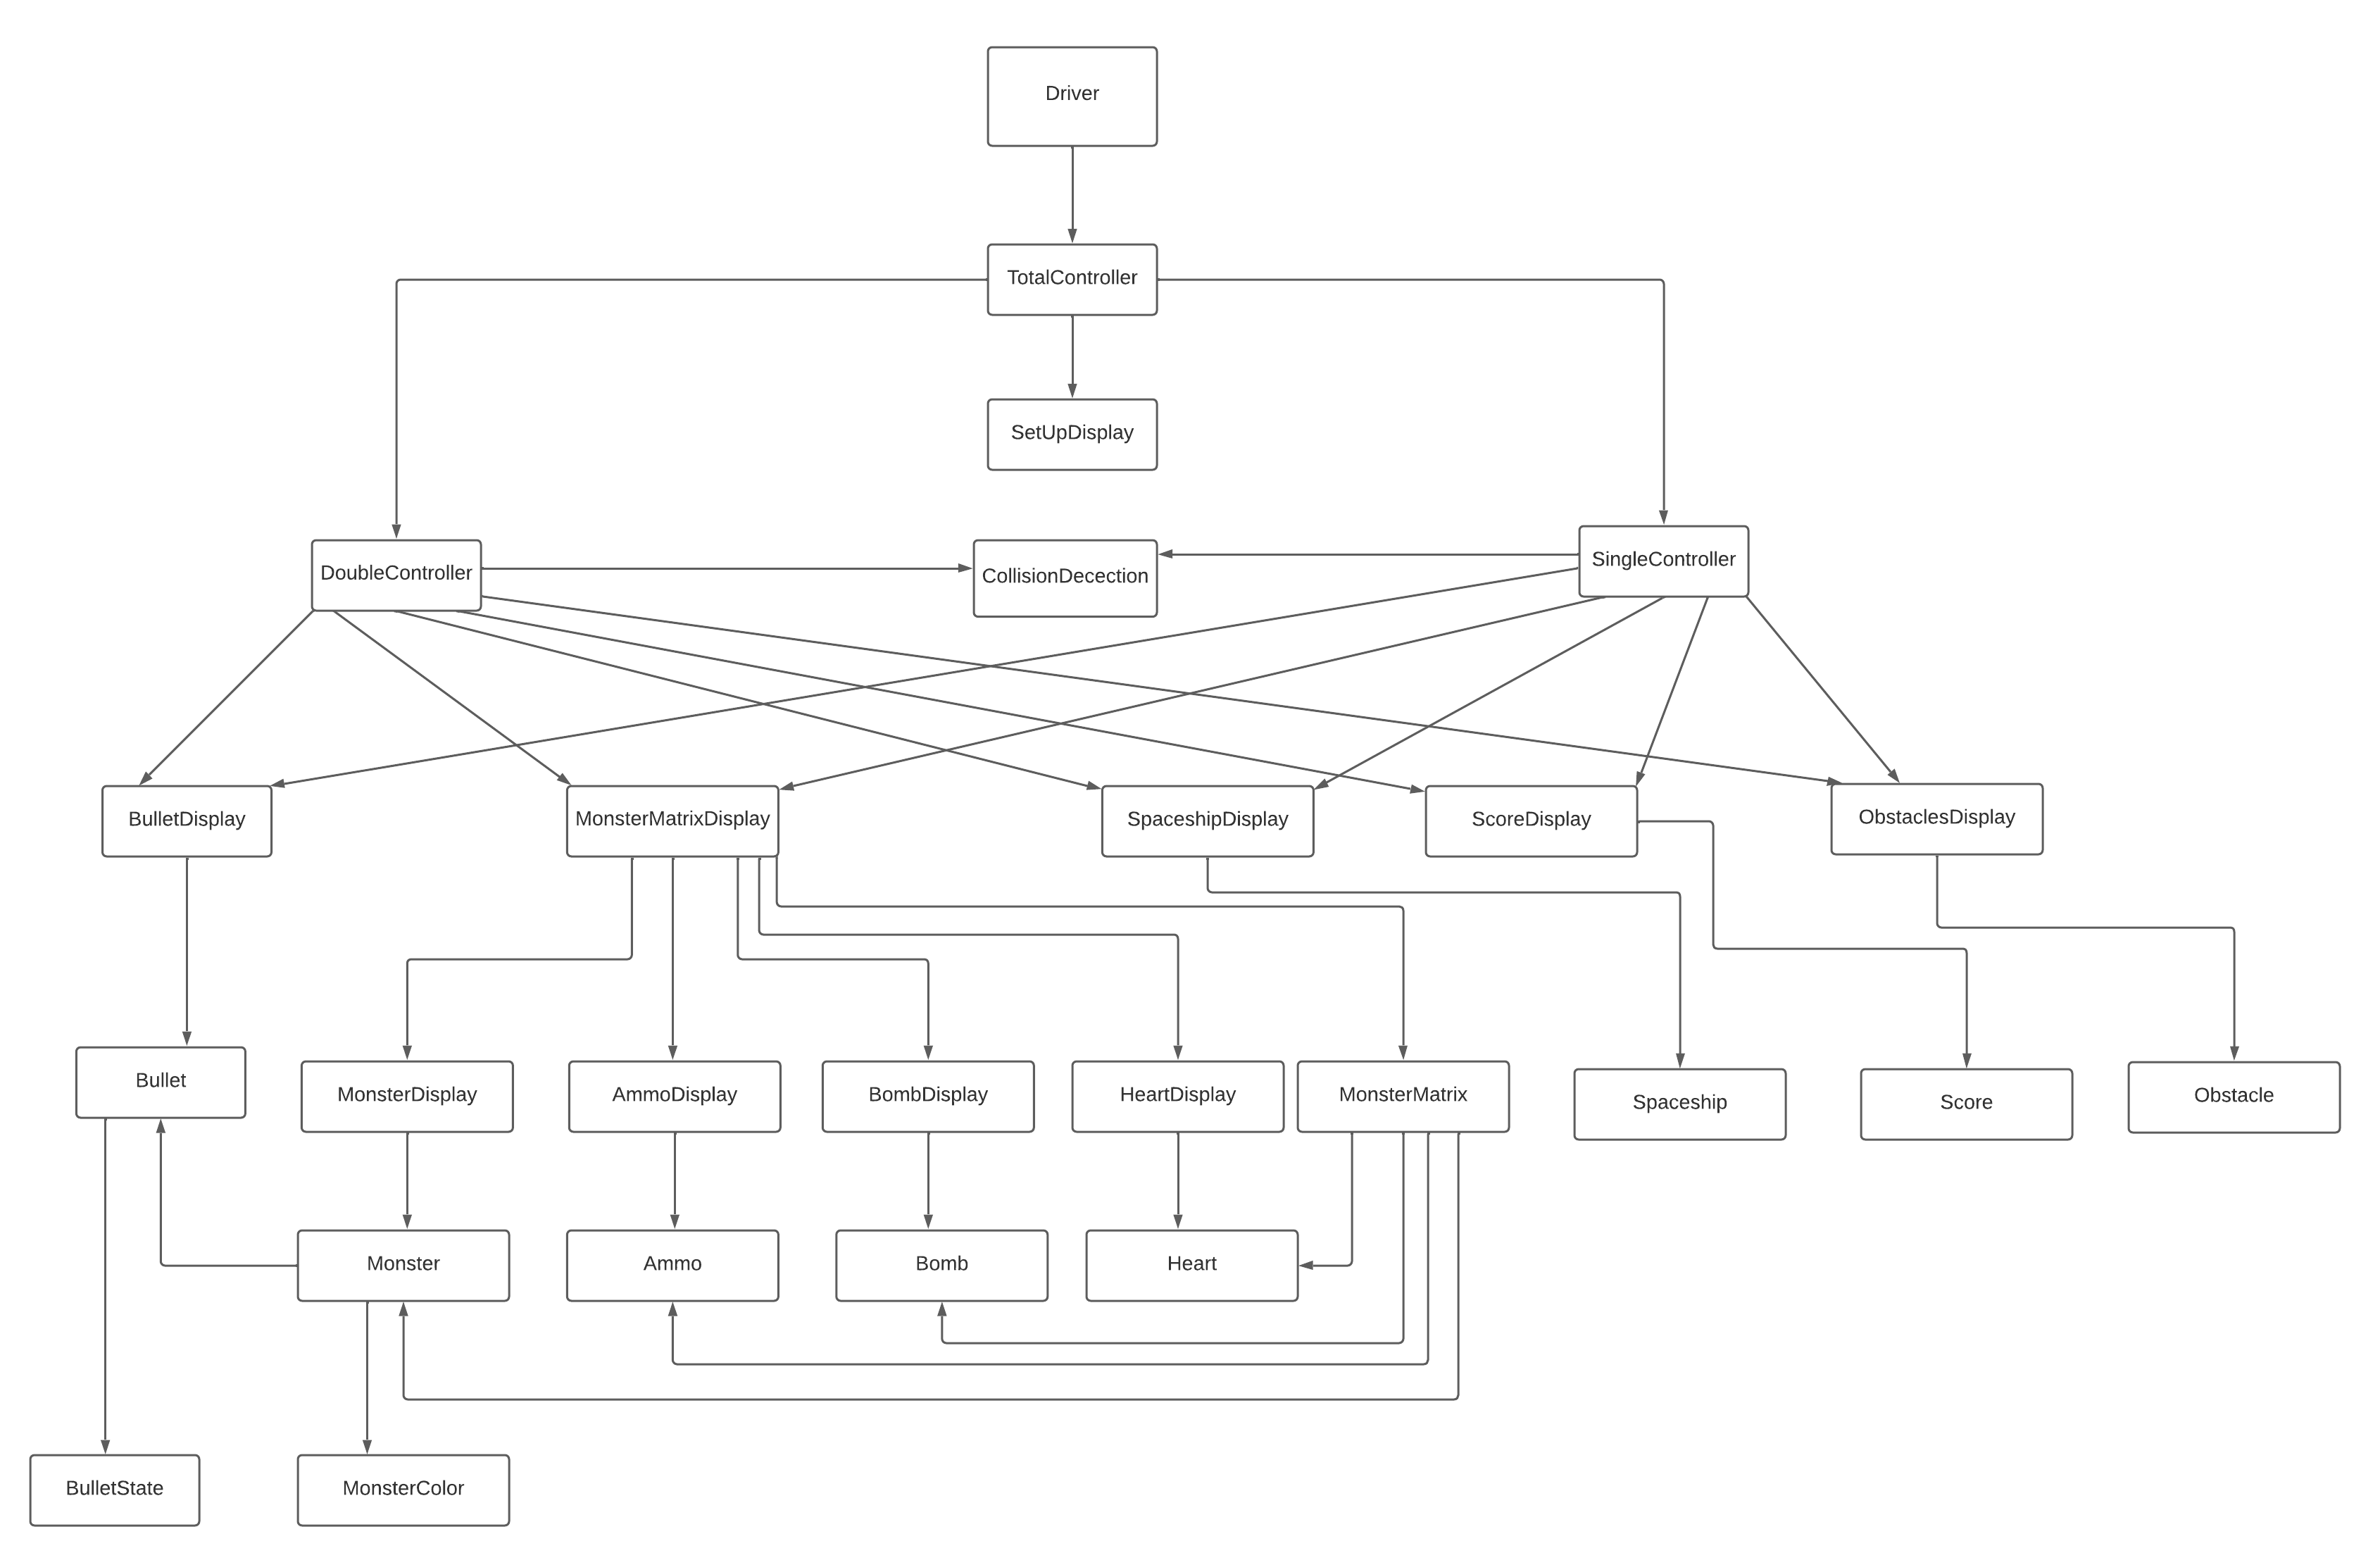
\includegraphics[scale = 0.35]{USE_H2.png}
\caption{Use hierarchy among modules}
\label{FigUH}
\end{figure}

\section{Gantt Chart}
For the gantt chart of testing plan, please access it by the 
following links:\\
\href{https://gitlab.cas.mcmaster.ca/shit19/2022_winter_3xa3_l03_g07/-/blob/main/ProjectSchedule/Gantt_Project_Design_Finished.gan}{\textcolor{red}{.gan file}}
\\
\href{https://gitlab.cas.mcmaster.ca/shit19/2022_winter_3xa3_l03_g07/-/blob/main/ProjectSchedule/Gantt_Project_Design_Finished.pdf}{\textcolor{red}{.pdf file}}

\section*{Reference}
David L. Parnas. On the criteria to be used in decomposing systems 
into modules. Coom.ACM, 15(2):1053-1058, December 1972.\\
David L. Parnas. Designing software for ease of extension and contraction. In ICSE '78: proceedings of the 3rd international conference on software engineering, pages 264-277, Piscataway, NJ, USA, 1978. IEEE Press. ISBN None.\\
D.L. Parnas, P.C. Clement, and D. M. Weiss. The modular structure
of complex systems. In international Conference on Software Engineering, pages 408-419, 1984.
\end {document}

